\documentclass{IEEEtran}

%\pagenumbering{roman}
\usepackage{xr}
\externaldocument{Classification}
\usepackage{cite}
\usepackage{amsmath}
\usepackage{tikz}
\usepackage{mathdots}
\usepackage{yhmath}
\usepackage{cancel}
\usepackage{color}
\usepackage{siunitx}
\usepackage{array}
\usepackage{multirow}
\usepackage{amssymb}
\usepackage{gensymb}
\usepackage{tabularx}
\usepackage{booktabs}
\usetikzlibrary{fadings}

\title{A Review of Techniques Related to Automated Facial Expression Recognition}
%\author{Austin Dase}
\author{\IEEEauthorblockN{Austin Dase}

\IEEEauthorblockA{Department of Computer and Information Sciences\\
Towson University\\
Towson, Maryland 21252\\
Email: adase1@students.towson.edu}}


\begin{document}

\maketitle

\tableofcontents

\section{Introduction}
The ability to recognize emotion displayed by the face is a critical part of human intelligence. This ability that is second-nature to humans is non-trivial for machines faced with the same task. Research has shown that humans can correctly identify expressions of emotion in facial images \cite{cecilione2017test} with a consistently high degree of accuracy while computers have historically struggled when faced with similar tasks. 

The goal of this paper is to survey the existing research that has been done on facial expression recognition in still images. Systems that have implemented facial expression recognition and that have implemented capabilities related to facial expression recognition are examined and reviewed. A robust facial expression recognition system at it's most basic level is an input-output system where inputs are images and outputs are the determined emotion expressed. In the following sections, three distinct modules that make up this type of system are examined: face detection, feature extraction, and classification. The first stage of a robust facial expression recognition system is determining if the image contains a face or not, this is the goal of the face detection module. Various methods for face detection are examined in \ref{FaceDetection}. If no face is detected then the system can cease processing. If a face is detected then the system can proceed with the second module, feature extraction. Feature extraction, examined in \ref{FeatureExtraction}, concerns itself with preparing the image data for the classification module. During the feature extraction stage, relevant data is extracted and transformed to help optimize the classification process. Because image files can have high volumes of extraneous data this phase is often concerned with reducing the volume of data that will be used to make a classification decision in order to improve performance. Finally, the classification module uses the output data from the feature extraction module to classify the emotion being expressed in the image. In \ref{classification}, methods for classification are examined.

The result of this paper will be a consolidation of methods and techniques that can be used as part of a robust system for facial expression recognition in images. Based on the findings of this work, in future work a system will be proposed, implemented, and compared against prior work in the field.

%\documentclass[12pt]{article}

%\usepackage{cite}

%\begin{document}

\section{Face Detection} \label{FaceDetection}
The first step in any system seeking to classify facial images is identifying the presence of a face in an image. The process of face detection involves two steps: determining if there is a face or not and then determining the boundaries of the face in the image. The primary challenge in the face detection stage is the trade-off between false positives/negatives and performance. In the following section, three techniques for detecting faces in images are presented: template models, geometric models and machine learning models.

\subsection{Template Models}

A method for detecting faces in images using template matching combined with support vector machines (SVM) is described in \cite{ai2001face}. Templates are used for identifying face candidate areas and a SVM classifier is used to classify candidate areas as face or non-face areas.

The first stage in the model described in \cite{ai2001face} is to utilize templates to filter out face candidate images for the classifier to analyze. Two templates are used for this stage: eyes-in-whole and face itself \cite{ai2001face}. The two templates were generated through analysis of a set of 50 mugshots that were aligned, normalized for size, and then averaged to create one image called the average face \cite{ai2001face}. The average face image is then sampled for two regions: the 20 x 20 whole face region and the 20 x 8 eyes-in-whole region \cite{ai2001face}. These templates are applied to the testing images by finding correlation coefficients for intensity for the test image related to the templates. Images where both templates match over a threshold of .25 are retained for SVM analysis \cite{ai2001face}.

The subset of images that are identified as face candidate images are then classified by a SVM as either containing a face or not. The SVM was trained on 5125 face sample images. In order to improve training speed and performance the negative training examples were collected using samples identified incorrectly by the template matching method \cite{ai2001face}. After training and testing once with incorrectly labeled images from template matching, all images incorrectly labeled by the SVM were subsequently used in the next iteration of training as negative examples \cite{ai2001face}. This process was then repeated until an appropriate number of negative samples were available for testing \cite{ai2001face}.

In order to detect faces of varying scale in the original image, a pyramid of images, each a sub-sample of a ratio of 1.2 to the next, was generated and filtered using template matching and SVM \cite{ai2001face}. 

% Unsure about this piece
%Because the authors felt that images that include faces tend to give high responses for consecutive scaled images, a 

For a test set of 230 images with a total of 545 faces, the algorithm described in \cite{ai2001face} detected 516 faces with a positive detection rate of 94.7\% and 815 false-positives. These results on the same test set compared with system 5 (single neural network) and system 11 (two neural networks) described by \cite{rowley1998nn} show that systems described by \cite{rowley1998nn} produce higher detection rates, 97.8\% and 96.3\% respectively. System 5 produces a much higher number of false-positives (1841) and System 11 produced a lower number of false positives (87).

The algorithm is also tested on the test set from \cite{rowley1998nn} which consists of 130 images with 507 faces. The template matching and SVM system detected 415 faces with a detection rate of 81.9\% and 465 false-positives. System 5 by \cite{rowley1998nn} detected 459 faces with a detection rate of 90.5\% and 570 false-positives. The System 11 by \cite{rowley1998nn} detected 437 faces with a detection rate of 86.2\% and 23 false-positives.

Overall the experimental results indicate that the template and SVM based system may be superior to System 5 proposed by \cite{rowley1998nn} and inferior to System 11 proposed by \cite{rowley1998nn}.

%The SVM's kernel function is the Gaussian radial basis function and 374 of the possible 400 points are used as input vectors \cite{ai2001face} ( some corner points are excluded). 


\subsection{Geometric Models}
A method for detecting faces in images using geometric rules is proposed by \cite{lin2000human}. In \cite{lin2000human} know geometric characteristics of facial feature are used during analysis to detect the presence of a face in an image. The first step in the processes outlined by \cite{lin2000human} is to read in the image and convert it to a binary image. The second step is to label all 4-connected components in the resulting images to form blocks of interest and then to determine the center of each of those blocks \cite{lin2000human}. The third step identifies all groups of three blocks whose centers form an isosceles triangle. Finally, all blocks that are part of triangles found in step three are labeled as potential face regions \cite{lin2000human}.

The binary conversion first transforms any color images to grayscale by eliminating hue and saturation and retaining luminance \cite{lin2000human}. All grayscale images are then thresholded (relying on the assumption that objects of interest are darker than the background) with a given threshold $T$. Morphological operations of erosion, then dilation (also called opening) are performed on the resulting binary images to remove noise followed by dilation and erosion (also called closing) to close holes.

Next, 4-connected components are identified in the image. Based on the idea that two eyes and a mouth will form an isosceles triangle \cite{lin2000human}, all sets of 4-connected blocks are then tested for conformance to rules, allowing for 25\% deviation, that the centers of the three blocks create an isosceles triangle. After all isosceles triangles are identified as potential face regions, they are verified using a combination of size normalization, weighted mask and threshold to determine if the potential face region is a verified face.

All identified potential face regions are normalized in size (pixel height and width) using bi-cubic interpolation \cite{lin2000human}. Based on the results of 10 binary training faces, the authors determined a target mask with which to compare candidate regions. Based on the similarity between the target mask and the mask obtained from the normalized face region, the region is classified as either a face region or a non-face region. The method for creating the target mask and for computing the weighted comparison is described in \cite{lin2000human}. 

Experimental results from testing the system described in \cite{lin2000human} showed that execution time for face detection varies based on size, resolution, and complexity of the images.


\subsection{Machine Learning Models}
\subsubsection{AdaBoost}
A method for face detection in images that attempts to balance performance with accuracy is described in \cite{viola2004robust}. By refining concepts from prior research and providing novel methods for calculation \cite{viola2004robust} attempt to achieve a more accurate system for face detection that improves performance over existing models.

The integral image concept is introduced by \cite{viola2004robust} as a method for pre-processing to improve performance. The integral image is created by scanning the image one time from left to right and generating an integral image where the value at each point $(x,\: y)$ in the integral image is equal to the sum of all points above and to the left of the point $(x,\: y)$ in the original image. This concept is expressed by \cite{viola2004robust} in the below formula where $ ii(x, \: y) $ represents a point on the integral image and $ i(x^\prime, \: y^\prime) $ represents a point on the original image:

\begin{equation}
\label{eqn_integralImage1}
ii(x, \: y) \; = \sum\limits_{x^\prime \, \leq \, x,\, y^\prime \, \leq \, y} i(x^\prime,\: y^\prime)
\end{equation}

After the integral image is created, it is used for computing values for rectangle features defined by \cite{viola2004robust}. The rectangle features are employed by \cite{viola2004robust} in an effort to improve performance over pixel-based classification methods. Three kinds of rectangle features are used: two-rectangle features, three-rectangle features, and four-rectangle features. Two-rectangle features represent the difference between the sum of two adjacent and equal-sized rectangular regions, three-rectangle features represent the sum of an inner rectangle subtracted from the sum of two adjacent and equal sized outer rectangles and four-rectangle features represent the difference in sums of diagonally adjacent and equal sized rectangles \cite{viola2004robust}.

A principal benefit of the integral image is the computational advantage it provides over other methods. Most face detection methods scan the image in search of faces at multiple scales. In the example provided by \cite{viola2004robust}, the  scale of 24 x 24 pixels is used for generating the first set of rectangle features. Next, the size of the rectangle features is increased by a factor of 1.25 and the rectangle features are recalculated. This process is repeated until the rectangle feature is too large for the image, the number of times given by:

\begin{equation}
\label{eqn_integralImage2}
min(x^\prime, y^\prime) = max(x, y) (S)^n
\end{equation}

\begin{equation}
\label{eqn_integralImage3}
n = \rceil{ \log_{S} max(x^\prime, y^\prime)}
\end{equation}

Where $S$ is the scaling factor of the rectangle features, $(x^\prime, y^\prime)$ are the dimensions in pixels of the image and $n$ is the number of iterations of scaling features to produce. 
%Further, the number of features produced at each iteration is given by Therefore, 
An image of size 384 x 288, starting with a base rectangle feature scale of 24 x 24 will produce 160,000 features for each image. Not only is this a large number of features, but the calculation required for each one is intensive and repetitive. \cite{viola2004robust} show that by using the integral image, the amount of computation necessary to compute each of these features is greatly reduced.

In order to perform classification, a variant of the AdaBoost algorithm used for feature selection is used \cite{viola2004robust}. For each feature, a weak learning algorithm first determines the optimal threshold of the classification function \cite{viola2004robust}.From there multiple rounds of weak learning classification are performed and finally result in a strong classifier that is the combination of all the weak classifiers \cite{viola2004robust}. The result is a classification of the region as either a face or a non-face region. 


\subsection{Neural Network Model}
A model using neural networks (NN) to detect the presence of a face in images is described in \cite{rowley1998nn}. The models proposed by \cite{rowley1998nn} utilizes multiple layers of neural networks to perform feature extraction and detection. In order to accommodate for the commonality of large variances in lighting, occlusion, pose, expression, and identity, \cite{rowley1998nn} states that multiple classifiers should be used to help handle these variations and that the output of those classifiers can be used as input into a final classifier that determines the presence of a face in the image.

The systems for face detection proposed by \cite{rowley1998nn} consists of 4 primary modules: localization and pose estimation, preprocessing, detection, and arbitration. Localization and pose estimation is performed with a neural network that analyzes the pixel values of the image as inputs. Localization determines the approximate boundary of the head in the image. Pose estimation determines the approximate angle of any tilt or roll from upright of the head in the image. Preporcessing is preformed using traditional image processing techniques for improving brightness and contrast as well as to reduce the impact of variations caused by lighting or camera quality \cite{rowley1998nn}. The detection phase, performed with a neural network, makes an initial determination as to whether there is a face in the region or not. Finally, arbitration is performed with another neural network that analyzes the results of prior stages to make the final determination if the face detected in other stages is valid or not.


The first system presented by \cite{rowley1998nn} is concerned with upright face detection. First, the image is segmented into regions of 20 x 20, 10 x 10, 5 x 5 and 20 x 5 pixels and those regions are fed to a neural network classifier that determines locations that might contain a face. This same process is repeated using a sub-sample of the original image and applying the detection networks again. The outputs of these networks are connected to a final arbitrator network that makes the determination as to whether or not the original 20 x 20 region contains a face \cite{rowley1998nn}.

The second system proposed by \cite{rowley1998nn} is concerned with tilted face detection. The system for upright detection is prepended with another neural network that detects the possible tilt or rotation of the face in the window and performs the necessary rotation to make the face upright for the face detector \cite{rowley1998nn}. Even if there is no face in the window, the rotation is still applied as the non-face window will still result in a non-face detection \cite{rowley1998nn}.

The systems proposed by \cite{rowley1998nn} both performed well on the testing data compared to prior techniques. The upright face detection system was evaluated with a testing data set of images compiled by the author as well as images from the FERET database that contain frontal faces. The tilted face detection system was evaluated using the same data set collected for the upright detection algorithm as well as images from the FERET database, classified into three groups based on how far the face in the image is aligned from the frontal position \cite{rowley1998nn}.


%$$ NEED \ MORE $$


%\bibliographystyle{ieeetr}
%\bibliography{references}


%\end{document}




%\documentclass[12pt]{article}

%\usepackage{cite}



%\begin{document}


\section{Feature Extraction and Selection} \label{FeatureExtraction}
In any facial expression recognition system there are at least two stages: feature extraction and classification \cite{lajevardi2012automatic}. In the feature extraction stage, features (also called attributes) are extracted from the raw image data and are subsequently used as input to the classification stage of the process. The quality of the feature extraction methodology therefore has a major impact on the ability of the classification stage to accurately identify the expression displayed in the original image \cite{lajevardi2012automatic}. Each of these two stages can be further decomposed into sub-modules and can be performed in a variety of ways. 

 In any automatic classification system, a major subset of the system will be concerned with extracting features from the raw data in a format that the classification algorithm can process successfully. The feature extraction process can be decomposed into two steps: feature construction and feature selection \cite{guyon2008feature}. Feature construction concerns itself mostly with transforming the raw data into a format that the system can process; features used as input to classification algorithms can be binary, continuous or categorical \cite{guyon2008feature}. Common feature construction methods include: standardization, normalization, signal enhancement, feature discretization, and non-linear expansion \cite{guyon2008feature}. Feature selection then analyzes the output of the feature construction process and selects the subset of information that will be used as features for classification. While feature selection's primary goal is to filter out noise by selecting the most relevant and informative features, it can also reduce the size of data that must be processed thereby improving algorithm performance and reducing storage requirements \cite{guyon2008feature}.

Construction of features from facial images generally takes one of two approaches: geometric feature-based or appearance-based \cite{tian2011facial}. Geometric feature-based approaches include information about the shape and location of facial components like the mouth, eyes, nose, and eyebrows. These components are represented as features that encode the geometric information each of the components for use in classification \cite{tian2011facial}. Appearance-based methods  apply image filters in order to extract relevant data for use in classification and focus on either the entire face or select regions of the face image without regard to the geometric location of the features \cite{tian2011facial}. 
 
After the feature set has been extracted, it is often necessary to select a subset of features for use in classification. There are two general techniques for feature selection: filter-based methods and wrapper or embedded based methods \cite{guyon2008feature}. Filter-based methods rank features by their relevance or importance to the classification model. Rankings are commonly produced by statistical analysis and do not provide any optimization for prediction performance \cite{guyon2008feature}. Wrapper, or embedded methods utilize a learning model for selection of an optimal feature subset. Features which have the strongest predictive power for the model are selected for use in classification. Embedded feature selection refers to analysis that is done during the training of a model \cite{guyon2008feature}.


Feature extraction and selection methods are examined by \cite{lajevardi2012automatic} in order to compare accuracy of different models. Models examined by \cite{lajevardi2012automatic} include Gabor filters, log Gabor filters, local binary pattern (LBP) operators, higher-order local autocorrelation (HLAC) and HLAC-like features (HLACLF). A system is proposed that includes pre-processing, face detection, facial feature detection, facial feature extraction, feature selection, training, and classification modules.  

The pre-processing module generates an image that is uniform in shape and size, has normalized intensity, and depicts a face expressing an emotion \cite{lajevardi2012automatic}. In order to detect the face area, the Viola-Jones method \cite{viola2004robust} is used. The result of the pre-processing is a new image of pixels that the face area detection determined are within the face area.

The methods for feature extraction use by \cite{lajevardi2012automatic} are appearance-based extraction methods. For feature selection, \cite{lajevardi2012automatic} employ both filter and wrapper based methods.
Mutual information selection seeks to select the features that have the most mutual information between the feature and the classes \cite{lajevardi2012automatic}.
Minimum redundancy seeks to select features that have the least amount of redundant information between each other \cite{lajevardi2012automatic}.
A wrapper based optimization approach where classification error is iteratively reduced by removing features at each iteration that have the least predictive power. This wrapper based approach identifies the subset of features that produces the smallest error when classifying the training set of data \cite{lajevardi2012automatic}.

A Naive Bayesian classifier is used for final classification for images from the Cohn-Kanaade database and a K-NN classifier was used for images from the JAFFE database.

The JAFFE and Cohn-Kanade database were used for experimental analysis. For each database, the subjects in the labeled images displayed one of six basic emotions: anger, disgust, fear, happy, sad, and surprise. Classes were each of these emotions as well as a neutral class. Accuracy for each feature extraction methods was compared based on the feature selection method used. For each combination of feature extraction and feature selection method, training and testing was performed three training/testing times and the average result was reported. There was no overlap between subjects in the training set and the testing set in order to ensure person-independent classification. 


%\subsection{Spatial Domain Feature Extraction}
\subsection{Facial Animation Parameters Extraction}
A robust feature detection method for facial expression recognition in video sequences is presented in \cite{ioannou2007robust}. 19 facial feature points are extracted based on facial animation parameters (FAP) related to the facial action coding system (FACS). In addition to feature extraction, a confidence factor for each extracted point was produced allowing the expression classification stage to take into consideration the quality of each of the extracted features \cite{ioannou2007robust}.

The initial phase of face detection identified face and non-face areas in the image through nonparametric discriminant analysis performed with a support vector machine\cite{ioannou2007robust}. A rectangle boundary of the face is produced and then segmented using anthropometric rules into three regions of interest that are considered candidate regions for the left eye/eyebrow, right eye/eyebrow and the mouth \cite{ioannou2007robust}. Feature extraction is performed on these candidate regions instead of the entire image for improved accuracy and performance.

The head in the image is rotated to an upright position after estimating the head roll rotation based on the position of the eyes relative to one another \cite{ioannou2007robust}. In order to calculate the the angle between the horizontal plane and the eye centers, the eyes and eye centers are identified using a multilayer perceptron network applied to both eye candidate regions independently to produce a template for the shape of the eyes. In subsequent frames, the template is matched to the image to identify the eye using sum of absolute differences \cite{ioannou2007robust}. After rotating the head to an upright position, the segmentation of the face into candidate regions for feature extraction is performed again.

The feature extraction stage from \cite{ioannou2007robust} utilized a series of masks to extract boundaries of the eyes, eyebrows, and mouth. The nose was also detected but used mainly for geometric reference of other features (the eyes should be above the nose and mouth below). In addition to boundary extraction, center point and corner features were determined. 

Eye boundary detection was performed with a combination of masks based on luminance and color information and an edge-based mask\cite{ioannou2007robust}. The first mask described by \cite{ioannou2007robust} is the luminance and color information mask. This mask attempts to identify the eye boundaries based on the iris center and relies on the assumption that the eyelids usually appear darker than the skin and are typically adjacent to the iris \cite{ioannou2007robust}. Each of the eye-candidate regions identified by the neural network are examined independently to create one of these masks for each eye-candidate region. The region is first dilated and then a luminance threshold $t^e_b$ is found by:

\begin{equation}
\label{eqn_lumThresh1}
t^e_b \; = \frac{1}{3}(2\langle f_c(L^e, M^e_{nn}) \rangle ) + min(L^e)),
\end{equation}


\begin{equation}
\label{eqn_integralImage2}
f_c(A,B) = \{c_{ij}\}, \; c_{ij} = \begin{cases}
a_{ij}, & b_{ij} \neq 0, \\ 
0, & b_{ij} = 0,
\end{cases}
\end{equation}

where $l^e$ is the luminance channel of the eye candidate area, $\langle \bullet \rangle\ $ is the average over the image area, and $min(X)$ is the minimum value of area $X$ \cite{ioannou2007robust}. After applying $t^e_b$ to $L^e$ a mask identifying the eyelashes and iris is derived. The iris point is found based on the thickness of the object detected in the mask and is determined as the point where the distance obtained from a distance transform for the object is maximized \cite{ioannou2007robust}.


After all intended features are extracted, they can be used for classification. A rule based classification system is described by \cite{ioannou2007robust} which is discussed in \ref{3-RBC}.

\subsection{Deep Attentive Multi-path Convolutional Neural Network}
A novel system for facial expression recognition, Deep Attentive Multi-path Convolutional Neural Network (DAM-CNN), is proposed by \cite{xie2019deep}. The system, consists of three modules: feature extraction, salient region determination and classification. Feature extraction is done with the VGG-Face network as proposed by \cite{parkhi2015deep}. Feature refinement and salient region determination is performed with the proposed attention-based Salient Expressional Region Descriptor (SERD)\cite{xie2019deep}. Classification is performed with the proposed Multi-Path Variation-Suppressing Network (MPVS-Net) \cite{xie2019deep}. Within the context of feature extraction the VGG-Face and the SERD models are the most relevant, the MVS-Net will be discussed further in \ref{3-LBC}.

%\subsubsection{Initial extraction with VGG-SERD}
Initial feature extraction in \cite{xie2019deep} is performed with the VGG-Face model described in \cite{parkhi2015deep}. The VGG-Face model is a Convolutional Neural Network (CNN) and a pre-trained VGG-Face network that was fine-tuned for feature extraction by mapping the last pooling layer of the network to features of size 7 x 7 x 512 \cite{xie2019deep} for use in the SERD stage.

Based on concepts of Facial Action Coding System (FACS) around facial action units (AU's) described by \cite{friesen1978facial}, \cite{xie2019deep} determined that different facial regions provide unequally weighted information about facial expression. For this reason, the SERD model is proposed to modify the VGG-Face model by identifying features produced by the VGG-Face model that provide the greatest amount of information about the facial expression. The SERD consists of a network that produces an attention mask that quantifies the importance of each position in the feature maps and weights the features accordingly for input into the classification module \cite{xie2019deep}.
By joining together the VGG-Face model and the SERD the researchers produce a model they call VGG-SERD which produces extracts features from images weighted according to their importance in expression recognition as determined by AU's as described by the FACS.


%$$ NEED \ MORE $$

\subsection{Precise Eye Center Detection} \label{FE1}
Feature extraction has also been done based on facial features and their known positions relative to one another. When this approach is taken, often the eyes are the first feature detected and other features (nose, mouth, eyebrows... etc.) are determined based on their known relative position to the eyes. A method for identifying the precise location of eye centers using color information is described in \cite{skodras2015precise}.

After face regions are detected and segmented into regions of interest using methods described by \cite{viola2004robust}, the regions of interest for each of the eyes are evaluated by the system proposed in \cite{skodras2015precise} to determine the precise center of the eye. The first stage of analysis uses color information to build the eye map. The eye map is built off of evaluation of the $YCbCr$ color space of the image. %ignoring the luminance information $Y$ as the luminance information is not helpful in identifying different skin regions \cite{viola2004robust}.
 A map $EyeMapc$  of the eye region is built using the $Cb$ and $Cr$ values of the $YCbCr$ color space where:
\begin{equation}
\label{eqn_EyeMapC}
EyeMapC = \frac{1}{3} \{(Cb)^2 + (\overline{Cr})^2 + (\frac{Cb}{Cr}) \}
\end{equation}
 
 with $Cb$ and $Cr$ normalized over the range [0, 1] and $\overline{Cr} = 1 - Cr$ \cite{skodras2015precise}. Large values in the resulting map indicate a large difference in the color of pixels which is indicative of a boundary between skin and eye. After obtaining the $EyeMapC$ information, the map is divided by the  $Y$ information from the $YCbCr$ space to emphasize the iris area which is typically the brightest area in $EyeMapC$ \cite{skodras2015precise}. To further emphasize the iris area, morphological operations with a circular structuring element are applied to derive $EyeMapI$ \cite{skodras2015precise}. As \cite{skodras2015precise} state that iris size does not significantly vary across humans, the expected proportion of the iris to the face is used to estimate the size of the iris in the image:
 
\begin{equation}
\label{eqn_EyeMapC}
EyeMapI = \frac{EyeMapC \oplus B1}{(Y\ominus B2) + \delta}
\end{equation}
 
 where $\oplus$ detonates gray-scale dilation and $\ominus$ detonates gray-scale erosion and:

\begin{equation}
\label{eqn_B1}
B1 = \frac{IrisRad}{2},
\end{equation}

\begin{equation}
\label{eqn_B2}
B2 = \frac{B1}{2},
\end{equation}

\begin{equation}
\label{eqn_IrisRad}
IrisRad = \frac{EyeRegionWidth}{10},
\end{equation}

\begin{equation}
\label{eqn_delta}
\delta = mean(Y \ominus B2 )
\end{equation}

\cite{skodras2015precise}

Based on the fact that the eye exhibits properties of symmetry, a radial symmetry transform is used to enhance the eye center location in both the luminance image as well as the \textsl{eye map}  by maximizing values at the eye center  \cite{skodras2015precise}. The maximum pixel value $(x_C,y_C)$ of the sum of the radial transformation of the luminance image as well as the radial transformation of the \textsl{eye map} ($C$) designates the estimated eye center location.

Performance of the system proposed by \cite{skodras2015precise} was evaluated using four publicly available database: the GTAV face database, the MUCT face database, the FERET face database and the BUHP database. The normalized error between estimated eye center and manually labeled eye center is used to evaluate the performance of the system on test images. Algorithm accuracy was expressed as the number of normalized errors that fell below an assigned threshold ( .25, .1, and .05), divided by the total number of images in the database \cite{skodras2015precise}. Results showed accurate estimation of eye center in cases when the eyes were not completely closed and when there was not extreme uneven illumination of the subject \cite{skodras2015precise}. For comparison, the algorithm proposed by \cite{skodras2015precise} was evaluated against results from other methods that had either been reported with the same dataset or where an implementation of the algorithm was publicly available. The proposed algorithm outperformed all algorithms compared to in almost every case showing that the proposed method provides a significant improvement over existing techniques \cite{skodras2015precise}.

\subsection{Face Recognition Using Spatiotemporal ICA and Euclidean Features}
A method combining Spatiotemporal Independent Component Analysis (ICA) and Euclidean Features for face recognition is proposed by \cite{lei2006combination}. In their work, \cite{lei2006combination} extract the distance between the centers of the eyes as well as the distance from the center of the left eye to the center of the mouth in order to create a ratio to scale the image. In order to determine these points, the eyes and mouth had to be identified in the image. For identification of the eyes a multi-step process was used. First candidate regions were identified by implementing a pattern matching algorithm that relied on the light to dark to light contrast of the pupils and eyelashes \cite{lei2006combination}. After identification, candidate regions were analyzed for conformance with known eye shape and size and the candidate regions most closely matching this were selected. Finally the center point of each extracted eye was determined by finding local maxima on approximately the same horizontal level in the two eyes \cite{lei2006combination}. The eye regions were then finalized by selecting all pixels within a pre-determined distance from the detected eye centers \cite{lei2006combination}.

The mouth was detected using edge detection algorithms and known characteristics of mouths. A kirsch edge detection filter was used to identify edges in the image and because mouths are one of the most contrasting features of the face, the mouth was one of the prominent objects highlighted by the edge detector \cite{lei2006combination}. Again, after initial edge detection, the candidate regions were analyzed for conformance to known size and shape characteristics of mouths and the best match was selected as the detected mouth \cite{lei2006combination}. 

After identifying the eyes and mouth, the measurements discussed above were calculated and used to scale the image in preparation for Spatial and Spatiotemporal ICA. Spatial ICA breaks down the input image into components by multiplying the original image pixel values as a matrix with varying equal sized weighting matrices and treating the results as features for analysis. In addition to Spatial ICA, Spatiotemporal ICA was also used by \cite{lei2006combination}, however because Spatiotemporal ICA involves analysis of a sequence of images it is less relevant to the current work analyzing single images. Finally, after using ICA for feature extraction, face recognition was performed using K-NN and SVM classifiers.  




\subsection{Eye Detection Using CNN and SVM}
An eye detection method based on convolutional neural networks (CNN) and support vector machines (SVM) is presented by \cite{yu2018eye}. Classifiers are applied to the image to detect and refine the eye positions in the image. The classification techniques described by \cite{yu2018eye} start with more coarse filtration methods and progressively utilize finer classification to determine the eye location \cite{yu2018eye}. The methods proposed by \cite{yu2018eye} were shown perform better than previously proposed methods, especially in situations where other detection methods have shown to have shortcomings \cite{yu2018eye}.

The eye detection technique proposed by \cite{yu2018eye} is a three layer system. The first layer is a eye variance filter (EVF). The EVF relies on the observation that the grey level intensity in the eye region is more drastic than in other areas of the face \cite{yu2018eye}. The EVF is constructed based on the intensity of 30 known eye images in the database. By averaging the variation in grey intensity of the 30 training images, a variance image is constructed that represents the average variance values for the 30 known eye images. After the variance image is calculated another 30 known eye images as well as 30 non-eye images are used from the database to calculate the EVF threshold. Each of the 60 images are analyzed for grey intensity variance and their individual variances are correlated with the variance image. A variance threshold is selected so that non eye-images would be discarded and eye images would not be discarded. After this training phase, the EVF is ready to scan new images and filter out non-eye images before moving to the feature extraction phase.

The feature extraction phase of the eye detection system proposed by \cite{yu2018eye} is performed by a CNN. Eye images identified by the EVF are used as the input to the CNN, because the images are 32 x 32 the input layer of the CNN has 1024 inputs. Each of these inputs then map to a smaller set of nodes as they move through the networks hidden layers. What is typically considered the output layer of a CNN is replaced in \cite{yu2018eye} by a SVM, however for training the CNN is treated independently from the SVM. The CNN is trained in a traditional method where the final layer of the CNN represents the classification and training is done until classification results converge for the network \cite{yu2018eye}. Once this traditional training is complete the output layer of the network, which consisted of just two neurons, is replaced by a SVM \cite{yu2018eye}. The inputs to the SVM are the outputs of the hidden layer of the CNN just before the output layer, in the case of \cite{yu2018eye} layer 5. At this point the SVM is trained using the output features from the CNN. The intent of this approach is to utilize each classifier for processes with which it handles best. The CNN is typically used for multi-class classification problems and the SVM is used mainly for solving two-class problems. By introducing the SVM as the last layer of the CNN, the multi-class information derived by the CNN can be used by the SVM to make the final two-class determination.

The system proposed by \cite{yu2018eye} was trained using images from multiple datasets including: the extended M2VTS dabatbase (XM2VTS), Psychological Image Collection at Stirling (PICS) face database, Japanese Female Facial Expression (JAFFE) face database, Milborrow/University of Cape Town (MUCT) face database, California Institute of Technology (Caltech) face database, Self-face database, and face images from Internet websites \cite{yu2018eye}. The system was then tested on images from separate datasets including the BioID, IMM, FERET, and ORL face databases \cite{yu2018eye}.

\subsection{Feature Extraction Using Linear Regression}
A method for feature extraction using gradient and Laplacian operators along with linear regression is proposed and analyzed in \cite{alazzawi2018performance}. A fundamental operation to the feature extraction process outlined by \cite{alazzawi2018performance} is edge detection. For this reason \cite{alazzawi2018performance} examined the performance of various edge detection operators: Sobel filter (SF), Prewitt filter (PF), Roberts filter (RF), zero cross filter (ZF), Laplacian of Gaussian filter (LG), and Canny filter(CF)\cite{alazzawi2018performance}. The various edge detection filters were combined with the slope of the linear regression (SLP) analysis and artificial neural networks for face recognition\cite{alazzawi2018performance}. While face recognition is a separate field from expression detection, there are many overlapping concepts between the fields. For this reason, the feature extraction methodology described in \cite{alazzawi2018performance} is of greatest relevance to the current work and will be discussed.

The first step in the face recognition algorithm proposed by \cite{alazzawi2018performance} is pre-processing and edge detection. The second step is image segmentation and feature extraction, and the third step is classification. During pre-processing, the face image is first scanned by the selected edge detection algorithm and then segmented into equal sized blocks and treated as a feature vector. Two groups of edge detectors are used: gradient based operators are SF, PF, and RF and Laplacian based operators are LF, ZF, and CF \cite{alazzawi2018performance}. After feature vectors have been created, the proposed SLP extraction method from \cite{alazzawi2018performance} is used to select features that are impacted least by outliers or noise. The SLP method is a unique method proposed by \cite{alazzawi2018performance}, for refining features found by edge detection. First in SLP, images are converted to binary using an edge detection filter then each image is divided into segments. Then for each segment, the pixels with values of 1 are considered points on the $(x, y)$ plane and regression is used to determine the equation for the line of best fit for the points. The slope of the line is then added to a matrix of the slopes of the lines from each of the other segments and the resulting matrix is used as the feature input to the classification algorithm \cite{alazzawi2018performance}.

Combination edge detector and feature extraction methods were tested by \cite{alazzawi2018performance} on the BIO OS database from \cite{bioid}. The experimental results of \cite{alazzawi2018performance} show that the number of segments is one of the most important parameters and that 100 total segments (10 horizontal and 10 vertical) is the optimal number of segments \cite{alazzawi2018performance}. Additionally, the optimal number of neurons in the hidden layers of the neural network is 30 \cite{alazzawi2018performance}. \cite{alazzawi2018performance} also found that the thresholds for the edge detecting algorithms were important to the classification process, however the optimal thresholds for each of the edge detection filters were determined in a separate experiment. Finally, the best performing system is the LoG, SLP and ANN combination with a weighted mean score of over 95\% \cite{alazzawi2018performance}.

%

%$$ NEED \ MORE $$



%-------- Analysis of \cite{alazzawi2018performance} %----------------


%-------------------------------------------------------------------

%\subsection{Frequency Domain Feature Extraction}

\subsection{Gabor Filters}
Feature extraction using features from the frequency domain as well as the spatial domain is examined in \cite{lajevardi2012automatic}. 

2D Gabor filters can provide information about an image in both the spatial and frequency domains depending on the filter used. Gabor filters have eight degrees of freedom including $(x,\:y)$ coordinates specifying the location of the filter in the spatial domain and $(u,\:v)$ coordinates in the frequency domain, these are the independent variables that can be modified to tune the Gabor filter \cite{daugman1985uncertainty}. \cite{lajevardi2012automatic} performed facial feature extraction using Gabor filters focused on the spatial domain and log Gabor filters in the frequency domain. Log Gabor filters are used to overcome the limitations of Gabor filters in obtaining broad spectral information with maximal spatial localization \cite{lajevardi2012automatic}. Based on the results reported by \cite{lajevardi2012automatic}, log Gabor filters were shown to have better accuracy detecting facial expressions than Gabor filters.
	The features extracted using log Gabor filters in \cite{lajevardi2012automatic} are intended to capture information about shape, motion, color, texture and spatial configuration of the face aligned at particular orientations. For feature extraction, \cite{lajevardi2012automatic} use a bank of Gabor filters with five frequencies and eight orientations. Filters are expressed in \cite{lajevardi2012automatic} and are convoluted with the original image to create Gabor features. The results of facial expression classification using, Gabor filters, log Gabor filters, local binary pattern, HLAC features, and HLACLF features are compared in \cite{lajevardi2012automatic}.
	

%$$ NEED \ MORE $$


%\bibliographystyle{ieeetr}
%\bibliography{references}


%\end{document}




\iffalse
\documentclass{IEEEtran}

%\pagenumbering{roman}

\usepackage{xr}
\externaldocument{Classification}
\usepackage{cite}
\usepackage{amsmath}
\usepackage{tikz}
\usepackage{mathdots}
\usepackage{yhmath}
\usepackage{cancel}
\usepackage{color}
\usepackage{siunitx}
\usepackage{array}
\usepackage{multirow}
\usepackage{amssymb}
\usepackage{gensymb}
\usepackage{tabularx}
\usepackage{booktabs}
\usetikzlibrary{fadings}


\begin{document}
\fi
\section{Facial Expression Classification} \label{classification}
The classification portion of a facial expression recognition system at it's most basic level will take features as inputs and based on those inputs will make a determination of the expression displayed in the image. The input features will be the output of the feature extraction and selection stage and the determined class will be one of a pre-provided set of possibilities. In general, this type of classification has been performed either with a rule based scheme or using supervised machine learning classification algorithms. In the following section, rule-based and machine learning based classification methods will be examined.


\subsection{Rule Based Classification} \label{3-RBC}
\subsubsection{Probabilistic Model} As part of their system for robust facial expression recognition \cite{ioannou2007robust} implement a rule based classification model.
Instead of using the six archetypal expressions described by \cite{ekman1987universals} a quadrants of emotions wheel is used to classify emotions. A rule based probabilistic measure is used to determine which emotion is described in the image. The rules used by \cite{ioannou2007robust} consist of ranges corresponding to high, medium, and low activation of the facial animation parameters detected by the extraction phase. Because it is possible that not all possible defined features could be extracted from an image, \cite{ioannou2007robust} designed rules to ensure that only features that are known with a high degree of confidence have a significant impact on classification and those features that are not extracted or are extracted with lower degrees of confidence have less of an impact on the classification decision \cite{ioannou2007robust}. Based on the calculations of the rules outlined in \cite{ioannou2007robust}, the emotion is determined based on the $(x,y)$ point on the plot of activation emotion space as described in \cite{ioannou2007robust}. The $x$ and $y$ coordinates are determined based on the rules outlined in \cite{ioannou2007robust}.


\subsection{Machine Learning Based Classification} \label{3-LBC}
\subsubsection{Naive Bayesian Classifier}
A Naive Bayesian (NB) classification algorithm is used by \cite{lajevardi2012automatic} to classify images based on the output of each of the afore mentioned feature extraction methods. Naive Bayesian classifiers are Bayesian networks where all attributes are assumed to be independent \cite{zhang2004optimality}. Despite the fact that this assumption, called conditional independence, is rarely true in real world situations (there is typically some interdependence or correlation among features), Naive Bayesian classifiers have been shown to perform well compared to other classification methods \cite{zhang2004optimality}.

Bayesian classifiers make a classification determination based on the results of an evaluation function that examines the probability of each class given values fore each feature and selects the class with the highest probability. The algorithm stores the conditional probability, sometimes called the weight, of each feature given the class and for each iteration of training the conditional probabilities of each class are updated based on the result. It is an important characteristic of the Bayesian classifiers that the algorithm assumes that the features are statistically independent \cite{langley1992analysis}. Because of the fact that in most real world scenarios features are not statistically independent, initial work assumed that this classification method might produce poor results \cite{zhang2004optimality} \cite{langley1992analysis}. However, as shown in \cite{zhang2004optimality} that is not the case, rather Naive Bayesian classifiers have been shown to produce results on par with more sophisticated classification algorithms \cite{zhang2004optimality}.


The Naive Bayesian classifier is a probabilistic based model. First the probability of each class $c$ is calculated based on the given feature set $X = (x_1,x_2,...,x_n)$ as:

\begin{equation}
\label{eqn_nb_pclassGivenFeat}
p(c|X) = \frac{p(X|c)\:p(c)}{p(X)}
\end{equation}

\begin{center}
where
\end{center}
\begin{equation}
\label{eqn_nb_pclassGivenFeat}
p(c) = \frac{Number \: of \: Samples \: in \: Class \: c}{Total \: Number \: of \: Samples}
\end{equation}

 \cite{lajevardi2012automatic} and $p(X)$ is equal for all classes and can therefore be ignored \cite{rish2001empirical}.


The evaluation function $p(X|c)$ accounts for the probability of each feature set $X$ given each class $c$. This is often called the conditional probability. The function for the conditional probability is given as:

\begin{equation}
\label{eqn_nb_cprob}
p(X|c) = \prod_{i=1}^n p(x_i|c)
\end{equation}

and the class $C$ is determined by the maximum value of $p(c|X)$ after evaluating all classes $c$ where the total number of classes $k$ is shown as:

\begin{equation}
\label{eqn_nb_classify}
C = max \{p(c_1|X),...,p(c_k|X)\}
\end{equation}

\subsubsection{Neural Network Classifier}
Neural networks are a popular machine learning algorithm used for multi-class classification problem. Neural networks have been used been used in Face Detection, Feature Extraction and Classification stages of other facial expression recognition systems with success. \cite{rowley1998nn} used neural networks for face detection, \cite{xie2019deep}, \cite{ioannou2007robust}, and \cite{yu2018eye} used neural networks for feature extraction and \cite{alazzawi2018performance} and \cite{parkhi2015deep} used neural networks for face recognition. 

Neural networks, modeled after the function of neurons in the human brain, are networks of connected nodes called perceptrons \cite{pal1992multilayer}. There is an input layer of nodes where each node corresponds to one feature of input, followed by one or more ``hidden'' layers of nodes that connect prior layers to the next with weighted connections, the final layer is the output layer which encodes the classification \cite{pal1992multilayer}.


\begin{figure}
\centering


\tikzset{every picture/.style={line width=0.75pt}} %set default line width to 0.75pt        

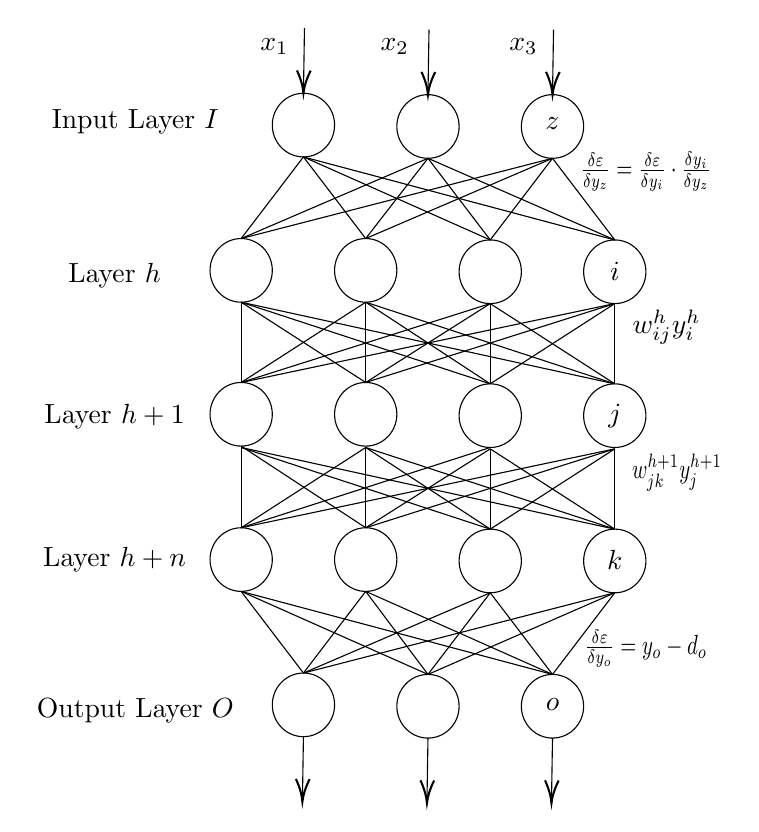
\begin{tikzpicture}[x=0.75pt,y=0.75pt,yscale=-1,xscale=1]
%uncomment if require: \path (0,918.3333435058594); %set diagram left start at 0, and has height of 918.3333435058594

%Flowchart: Connector [id:dp1999782616308523] 
\draw   (140,72.67) .. controls (140,64.2) and (146.72,57.33) .. (155,57.33) .. controls (163.28,57.33) and (170,64.2) .. (170,72.67) .. controls (170,81.14) and (163.28,88) .. (155,88) .. controls (146.72,88) and (140,81.14) .. (140,72.67) -- cycle ;
%Flowchart: Connector [id:dp4638526881382943] 
\draw   (200,73.33) .. controls (200,64.86) and (206.72,58) .. (215,58) .. controls (223.28,58) and (230,64.86) .. (230,73.33) .. controls (230,81.8) and (223.28,88.67) .. (215,88.67) .. controls (206.72,88.67) and (200,81.8) .. (200,73.33) -- cycle ;
%Flowchart: Connector [id:dp34953252838292914] 
\draw   (260,73.33) .. controls (260,64.86) and (266.72,58) .. (275,58) .. controls (283.28,58) and (290,64.86) .. (290,73.33) .. controls (290,81.8) and (283.28,88.67) .. (275,88.67) .. controls (266.72,88.67) and (260,81.8) .. (260,73.33) -- cycle ;
%Flowchart: Connector [id:dp8088598815308989] 
\draw   (110,142.67) .. controls (110,134.2) and (116.72,127.33) .. (125,127.33) .. controls (133.28,127.33) and (140,134.2) .. (140,142.67) .. controls (140,151.14) and (133.28,158) .. (125,158) .. controls (116.72,158) and (110,151.14) .. (110,142.67) -- cycle ;
%Flowchart: Connector [id:dp8319087784289663] 
\draw   (170,142.67) .. controls (170,134.2) and (176.72,127.33) .. (185,127.33) .. controls (193.28,127.33) and (200,134.2) .. (200,142.67) .. controls (200,151.14) and (193.28,158) .. (185,158) .. controls (176.72,158) and (170,151.14) .. (170,142.67) -- cycle ;
%Flowchart: Connector [id:dp08077051351305586] 
\draw   (230,143.33) .. controls (230,134.86) and (236.72,128) .. (245,128) .. controls (253.28,128) and (260,134.86) .. (260,143.33) .. controls (260,151.8) and (253.28,158.67) .. (245,158.67) .. controls (236.72,158.67) and (230,151.8) .. (230,143.33) -- cycle ;
%Flowchart: Connector [id:dp39097424978035744] 
\draw   (290,143.33) .. controls (290,134.86) and (296.72,128) .. (305,128) .. controls (313.28,128) and (320,134.86) .. (320,143.33) .. controls (320,151.8) and (313.28,158.67) .. (305,158.67) .. controls (296.72,158.67) and (290,151.8) .. (290,143.33) -- cycle ;
%Flowchart: Connector [id:dp16069978515034533] 
\draw   (110,212) .. controls (110,203.53) and (116.72,196.67) .. (125,196.67) .. controls (133.28,196.67) and (140,203.53) .. (140,212) .. controls (140,220.47) and (133.28,227.33) .. (125,227.33) .. controls (116.72,227.33) and (110,220.47) .. (110,212) -- cycle ;
%Flowchart: Connector [id:dp9151618610910661] 
\draw   (170,212) .. controls (170,203.53) and (176.72,196.67) .. (185,196.67) .. controls (193.28,196.67) and (200,203.53) .. (200,212) .. controls (200,220.47) and (193.28,227.33) .. (185,227.33) .. controls (176.72,227.33) and (170,220.47) .. (170,212) -- cycle ;
%Flowchart: Connector [id:dp3662992262656779] 
\draw   (230,212.67) .. controls (230,204.2) and (236.72,197.33) .. (245,197.33) .. controls (253.28,197.33) and (260,204.2) .. (260,212.67) .. controls (260,221.14) and (253.28,228) .. (245,228) .. controls (236.72,228) and (230,221.14) .. (230,212.67) -- cycle ;
%Flowchart: Connector [id:dp9663626257935529] 
\draw   (290,212.67) .. controls (290,204.2) and (296.72,197.33) .. (305,197.33) .. controls (313.28,197.33) and (320,204.2) .. (320,212.67) .. controls (320,221.14) and (313.28,228) .. (305,228) .. controls (296.72,228) and (290,221.14) .. (290,212.67) -- cycle ;
%Flowchart: Connector [id:dp43857777178268953] 
\draw   (110,282) .. controls (110,273.53) and (116.72,266.67) .. (125,266.67) .. controls (133.28,266.67) and (140,273.53) .. (140,282) .. controls (140,290.47) and (133.28,297.33) .. (125,297.33) .. controls (116.72,297.33) and (110,290.47) .. (110,282) -- cycle ;
%Flowchart: Connector [id:dp650814973856433] 
\draw   (170,282) .. controls (170,273.53) and (176.72,266.67) .. (185,266.67) .. controls (193.28,266.67) and (200,273.53) .. (200,282) .. controls (200,290.47) and (193.28,297.33) .. (185,297.33) .. controls (176.72,297.33) and (170,290.47) .. (170,282) -- cycle ;
%Flowchart: Connector [id:dp5987637413592404] 
\draw   (230,282.67) .. controls (230,274.2) and (236.72,267.33) .. (245,267.33) .. controls (253.28,267.33) and (260,274.2) .. (260,282.67) .. controls (260,291.14) and (253.28,298) .. (245,298) .. controls (236.72,298) and (230,291.14) .. (230,282.67) -- cycle ;
%Flowchart: Connector [id:dp7896686745607286] 
\draw   (290,282.67) .. controls (290,274.2) and (296.72,267.33) .. (305,267.33) .. controls (313.28,267.33) and (320,274.2) .. (320,282.67) .. controls (320,291.14) and (313.28,298) .. (305,298) .. controls (296.72,298) and (290,291.14) .. (290,282.67) -- cycle ;
%Flowchart: Connector [id:dp1684405299484435] 
\draw   (140,352) .. controls (140,343.53) and (146.72,336.67) .. (155,336.67) .. controls (163.28,336.67) and (170,343.53) .. (170,352) .. controls (170,360.47) and (163.28,367.33) .. (155,367.33) .. controls (146.72,367.33) and (140,360.47) .. (140,352) -- cycle ;
%Flowchart: Connector [id:dp4455266057616105] 
\draw   (200,352.67) .. controls (200,344.2) and (206.72,337.33) .. (215,337.33) .. controls (223.28,337.33) and (230,344.2) .. (230,352.67) .. controls (230,361.14) and (223.28,368) .. (215,368) .. controls (206.72,368) and (200,361.14) .. (200,352.67) -- cycle ;
%Flowchart: Connector [id:dp7841543637598003] 
\draw   (260,352.67) .. controls (260,344.2) and (266.72,337.33) .. (275,337.33) .. controls (283.28,337.33) and (290,344.2) .. (290,352.67) .. controls (290,361.14) and (283.28,368) .. (275,368) .. controls (266.72,368) and (260,361.14) .. (260,352.67) -- cycle ;
%Straight Lines [id:da7296614712186866] 
\draw    (155,88) -- (305,128) ;


%Straight Lines [id:da95549702416122] 
\draw    (155,88) -- (245,128) ;


%Straight Lines [id:da31187192688984444] 
\draw    (155,88) -- (185,127.33) ;


%Straight Lines [id:da0015227165925528752] 
\draw    (155,88) -- (125,127.33) ;


%Straight Lines [id:da795209449448232] 
\draw    (215,88.67) -- (305,128) ;


%Straight Lines [id:da640811476633236] 
\draw    (215,88.67) -- (245,128) ;


%Straight Lines [id:da10656368843132613] 
\draw    (185,127.33) -- (215,88.67) ;


%Straight Lines [id:da9817044619174213] 
\draw    (125,127.33) -- (215,88.67) ;


%Straight Lines [id:da16802623039360554] 
\draw    (275,88.67) -- (305,128) ;


%Straight Lines [id:da2864597359556491] 
\draw    (245,128) -- (275,88.67) ;


%Straight Lines [id:da34330068305222183] 
\draw    (185,127.33) -- (275,88.67) ;


%Straight Lines [id:da1424082061266967] 
\draw    (125,127.33) -- (275,88.67) ;


%Straight Lines [id:da9074039317146441] 
\draw    (125,158) -- (305,197.33) ;


%Straight Lines [id:da11181766109306235] 
\draw    (125,158) -- (245,197.33) ;


%Straight Lines [id:da09207421728387355] 
\draw    (125,158) -- (185,196.67) ;


%Straight Lines [id:da9269227384207284] 
\draw    (125,158) -- (125,196.67) ;


%Straight Lines [id:da6311242197193294] 
\draw    (185,158) -- (305,197.33) ;


%Straight Lines [id:da7157468882618694] 
\draw    (185,158) -- (245,197.33) ;


%Straight Lines [id:da8211510400805617] 
\draw    (185,158) -- (185,196.67) ;


%Straight Lines [id:da4109257013165539] 
\draw    (125,196.67) -- (185,158) ;


%Straight Lines [id:da7823810278397867] 
\draw    (245,158.67) -- (305,197.33) ;


%Straight Lines [id:da46603858418459443] 
\draw    (245,158.67) -- (245,197.33) ;


%Straight Lines [id:da4577071036682243] 
\draw    (185,196.67) -- (245,158.67) ;


%Straight Lines [id:da18689530464740267] 
\draw    (125,196.67) -- (245,158.67) ;


%Straight Lines [id:da33821056740652056] 
\draw    (305,158.67) -- (305,197.33) ;


%Straight Lines [id:da2773851803950296] 
\draw    (245,197.33) -- (305,158.67) ;


%Straight Lines [id:da7150342703655499] 
\draw    (185,196.67) -- (305,158.67) ;


%Straight Lines [id:da8985268693084112] 
\draw    (125,196.67) -- (305,158.67) ;


%Straight Lines [id:da7202780883807927] 
\draw    (125,228) -- (305,267.33) ;


%Straight Lines [id:da6556929946494692] 
\draw    (125,228) -- (245,267.33) ;


%Straight Lines [id:da8424315192219356] 
\draw    (125,227.33) -- (185,266.67) ;


%Straight Lines [id:da030649836950903175] 
\draw    (125,227.33) -- (125,266.67) ;


%Straight Lines [id:da10601673057451544] 
\draw    (185,228) -- (305,267.33) ;


%Straight Lines [id:da02545107643660449] 
\draw    (185,228) -- (245,267.33) ;


%Straight Lines [id:da29662255491602596] 
\draw    (185,228) -- (185,266.67) ;


%Straight Lines [id:da95922252204627] 
\draw    (125,266.67) -- (185,228) ;


%Straight Lines [id:da1410434965434737] 
\draw    (245,228.67) -- (305,267.33) ;


%Straight Lines [id:da8521452004546188] 
\draw    (245,228.67) -- (245,267.33) ;


%Straight Lines [id:da19151816481183603] 
\draw    (185,266.67) -- (245,228.67) ;


%Straight Lines [id:da5052208204128217] 
\draw    (125,266.67) -- (245,228) ;


%Straight Lines [id:da6133383723546693] 
\draw    (305,228.67) -- (305,267.33) ;


%Straight Lines [id:da17539038541864382] 
\draw    (245,267.33) -- (305,228.67) ;


%Straight Lines [id:da30035936693068677] 
\draw    (185,266.67) -- (305,228.67) ;


%Straight Lines [id:da9895102518248726] 
\draw    (125,266.67) -- (305,228.67) ;


%Straight Lines [id:da6150538084278878] 
\draw    (185,297.33) -- (155,336.67) ;


%Straight Lines [id:da15645548600782333] 
\draw    (245,298) -- (215,337.33) ;


%Straight Lines [id:da47973555385230315] 
\draw    (305,298) -- (275,337.33) ;


%Straight Lines [id:da6224422655891633] 
\draw    (185,297.33) -- (215,337.33) ;


%Straight Lines [id:da23891192060765398] 
\draw    (125,297.33) -- (155,336.67) ;


%Straight Lines [id:da0505740352889561] 
\draw    (245,298) -- (275,337.33) ;


%Straight Lines [id:da2663335492521943] 
\draw    (305,298) -- (215,337.33) ;


%Straight Lines [id:da3712812632879081] 
\draw    (125,297.33) -- (215,337.33) ;


%Straight Lines [id:da8197780144177969] 
\draw    (125,297.33) -- (275,337.33) ;


%Straight Lines [id:da8690041946805536] 
\draw    (305,298) -- (155,336.67) ;


%Straight Lines [id:da7488920028460424] 
\draw    (245,298) -- (155,336.67) ;


%Straight Lines [id:da8061753391239372] 
\draw    (185,297.33) -- (275,337.33) ;


%Straight Lines [id:da9063266102748762] 
\draw    (155.5,26) -- (155.03,55.33) ;
\draw [shift={(155,57.33)}, rotate = 270.90999999999997] [color={rgb, 255:red, 0; green, 0; blue, 0 }  ][line width=0.75]    (10.93,-3.29) .. controls (6.95,-1.4) and (3.31,-0.3) .. (0,0) .. controls (3.31,0.3) and (6.95,1.4) .. (10.93,3.29)   ;

%Straight Lines [id:da8634456062529243] 
\draw    (215.5,26.67) -- (215.03,56) ;
\draw [shift={(215,58)}, rotate = 270.90999999999997] [color={rgb, 255:red, 0; green, 0; blue, 0 }  ][line width=0.75]    (10.93,-3.29) .. controls (6.95,-1.4) and (3.31,-0.3) .. (0,0) .. controls (3.31,0.3) and (6.95,1.4) .. (10.93,3.29)   ;

%Straight Lines [id:da25580778693011763] 
\draw    (275.5,26.67) -- (275.03,56) ;
\draw [shift={(275,58)}, rotate = 270.90999999999997] [color={rgb, 255:red, 0; green, 0; blue, 0 }  ][line width=0.75]    (10.93,-3.29) .. controls (6.95,-1.4) and (3.31,-0.3) .. (0,0) .. controls (3.31,0.3) and (6.95,1.4) .. (10.93,3.29)   ;

%Straight Lines [id:da14598029696148118] 
\draw    (155,367.33) -- (154.53,396.67) ;
\draw [shift={(154.5,398.67)}, rotate = 270.90999999999997] [color={rgb, 255:red, 0; green, 0; blue, 0 }  ][line width=0.75]    (10.93,-3.29) .. controls (6.95,-1.4) and (3.31,-0.3) .. (0,0) .. controls (3.31,0.3) and (6.95,1.4) .. (10.93,3.29)   ;

%Straight Lines [id:da06438121952682252] 
\draw    (215,368) -- (214.53,397.33) ;
\draw [shift={(214.5,399.33)}, rotate = 270.90999999999997] [color={rgb, 255:red, 0; green, 0; blue, 0 }  ][line width=0.75]    (10.93,-3.29) .. controls (6.95,-1.4) and (3.31,-0.3) .. (0,0) .. controls (3.31,0.3) and (6.95,1.4) .. (10.93,3.29)   ;

%Straight Lines [id:da9952813591787621] 
\draw    (275,368) -- (274.53,397.33) ;
\draw [shift={(274.5,399.33)}, rotate = 270.90999999999997] [color={rgb, 255:red, 0; green, 0; blue, 0 }  ][line width=0.75]    (10.93,-3.29) .. controls (6.95,-1.4) and (3.31,-0.3) .. (0,0) .. controls (3.31,0.3) and (6.95,1.4) .. (10.93,3.29)   ;


% Text Node
\draw (121,39) node  [align=left] {};
% Text Node
\draw (64,145) node  [align=left] {Layer $h$};
% Text Node
\draw (64,213) node  [align=left] {Layer $h + 1$};
% Text Node
\draw (64,282) node  [align=left] {Layer $h + n$};
% Text Node
\draw (141,35) node  [align=left] {$x_1$};
% Text Node
\draw (199,35) node  [align=left] {$x_2$};
% Text Node
\draw (261,35) node  [align=left] {$x_3$};
% Text Node
\draw (74,71) node  [align=left] {Input Layer $I$};
% Text Node
\draw (74,355) node  [align=left] {Output Layer $O$};
% Text Node
\draw (275,352) node  [align=left] { $o$};
% Text Node
\draw (305,282.01) node  [align=left] { $k$};
% Text Node
\draw (305,212.67) node  [align=left] { $j$};
% Text Node
\draw (305,143.33) node  [align=left] { $i$};
\draw (275,72) node  [align=left] { $z$};
% Text Node
%\draw (345,177) node   {$w^{h}_{ij} y^{h}_{i} - \theta ^{h+1}_{j}$};

%\draw (320,25) node   {\scalebox{0.75}[1.0]{$\frac{\delta E}{\delta y_i} = \sum_{k \sigma} w_jk \frac{\delta E }{\delta z_k}$}};
\draw (320,95) node   {\scalebox{0.75}[1.0]{$\frac{\delta \varepsilon}{\delta y_z} = \frac{\delta \varepsilon}{\delta y_i} \cdot \frac{\delta y_i}{\delta y_z}$}};
\draw (330,170) node   {$w^{h}_{ij} y^{h}_{i}$};
\draw (335,240) node   {\scalebox{0.75}[1.0]{$w^{h+1}_{jk} y^{h+1}_{j}$}};
\draw (320,325) node   {\scalebox{0.75}[1.0]{$\frac{\delta \varepsilon}{\delta y_o} = y_o - d_o$}};


%\draw (335,192) node   {$- \theta ^{h+1}_{j}$};

% Text Node
%\draw (360,190) node   {$w^{h}_{ij} y^{h}_{i} - \theta ^{h+1}_{j}$};


\end{tikzpicture}

\caption{A Neural Network with $n + 1$ hidden layers, neuron outputs $y$ and connection weights $w$.}
\label{fig_sim}
\end{figure}


Given node $i$ in layer $h$ connected to node $j$ in layer $h+1$, the equation for the input ($x$) to $j$ from $i$ is given as the product of the output of $i$ and the weight of the connection from $i$ to $j$:

%\begin{equation}
%\label{eqn_nn_nodeinput}
% x^{h+1}_{j} \ = \ y^h_i w^h_{ij} - \theta^{h+1}_i
%\end{equation}
%$\theta^{h+1}_j$ is the threshold of neuron $i$ in layer $h$,

\begin{equation}
\label{eqn_nn_nodeinput}
 x^{h+1}_{j} \ = \ y^h_i w^h_{ij}
\end{equation}

or

\begin{equation}
\label{eqn_nn_nodeinput2}
 x_{j} \ = \ y_i w_{ij}
\end{equation}

where $y^h_i$ is the output of neuron $i$ and $w^h_{ij}$ is the weight of the connection between $i$ and $j$. $y^h_i$ is defined for nodes in the input layer $I$ as:

\begin{equation}
\label{eqn_nn_inodeoutput}
 y_j^I = x_j^I
\end{equation}

and for nodes in all other layers $h$ as:

\begin{equation}
\label{eqn_nn_hnodeoutput}
y^h_j = f(x_j^h)
\end{equation}

where $f(x_j^h)$ is the activation function. The most popular activation functions are the logistic sigmoid function, the hyberbolic tangent function (tanh) and the rectified
linear unit (ReLU) function \cite{lecun2015deep}. Currently the most popular of these activation functions is the ReLU function\cite{lecun2015deep}.

The logistic sigmoid function is given as:

\begin{equation}
\label{eqn_nn_sigmoid}
f(x) = \frac{1}{1 + e^{-x}}
\end{equation}

the hyberbolic tangent is given as:

\begin{equation}
\label{eqn_nn_tanh}
f(x) = \frac{e^x - e^{-x}}{e^x + e^{-x}}
\end{equation}

and the ReLu function is given as:
\begin{equation}
\label{eqn_nn_relu}
f(x) = max(0,x)
\end{equation}


Subsequentially the input to node $j$ in layer $h+1$ from $n$ nodes in layer $h$ that connect to $j$ is given by:

\begin{equation}
\label{eqn_nn_allnodeoutput}
x^{h+1}_{j} \ = \sum^n_{k=1} \ y^h_k w^h_{kj} - \theta^{h+1}_j
\end{equation}

where $ \theta^{h+1}_j $ is the threshold of neuron $j$ in layer $h+1$.



While data flows from the input layer of the network to the output layer, learning flows from the output layer to the input. During training, the weights of each connection are adjusted automatically to minimize the error between the expected output of any node and its actual output. This can be thought of as a relationship that indicates the magnitude of the impact of a change in weight on the error for that node \cite{lecun2015deep}. The weights for each node are adjusted based on the derivative of the cumulative error at each of the nodes in layers closer to the the output side of the network. Therefore the flow of the weight adjustments is in the opposite direction as the flow of data through the network, for this reason, this flow is called backpropogation \cite{lecun2015deep}.

Backpropogation begins at the output layer of the network where error for each node is calculated based on a selected cost function. Two commonly used cost functions are logistic regression and quadratic.

%\subsubsection{Quadratic Cost Function}
The quadratic cost function is the more simple of the two and has been used in some of the earliest neural networks \cite{rumelhart1988learning}. Where error $\varepsilon$ at one node $o$ is given by:

\begin{equation}
\label{eqn_nn_error}
\varepsilon_o = \frac{1}{2} (y_o - d_o)^2
\end{equation}

And where error of the entire network can be expressed as:
\begin{equation}
\label{eqn_nn_total error}
\varepsilon = \frac{1}{2}\sum^m_{h=1} \sum^{N_L}_{j=1} (y_j - d_j)^2
\end{equation}
where $m$ is the total number of layers in the network and $N_L$ is equal to the number of nodes in the current layer $h$.

Error at a node can be minimized using gradient decent by differentiating equation \ref{eqn_nn_error} \cite{rumelhart1988learning}, this gives:

\begin{equation}
\label{eqn_nn_errordiff}
\frac{\delta \varepsilon}{\delta y_o} = y_o - d_o
\end{equation}

Then based on the chain rule \cite{abdeljawad2015conformable}, the value of $\frac{\delta \varepsilon}{\delta y_k}$ for any node $k$ connected to node $o$, where $o$ is one layer closer to the output layer than $k$, can be given as:
\begin{equation}
\label{eqn_nn_errordiffchain}
\frac{\delta \varepsilon}{\delta y_k} = \frac{\delta \varepsilon}{\delta y_o} \cdot \frac{\delta y_o}{\delta y_k}
\end{equation}



Because we cannot directly modify the output of a node $k$ based on error for the output of node $o$ which is in the layer above it, based on the relationship from equation \ref{eqn_nn_nodeinput}, the input to node $o$ can be indirectly modified by adjusting the weight of the connection between $k$ and $o$.
%The input to node $i$ from node $z$ ($x_{zi}$) can be given as: $$ x_{zi} = y_z w_{zi} $$


Therefore we can adjust the input to $o$ from $k$ by adjusting the value of $w_{ko}$ instead of $y_k$. This gives us equation \ref{eqn_nn_errordiffchain} expressed in terms of the weight of the connection between nodes $k$ and $o$:

\begin{equation}
\label{eqn_nn_weightdiff}
\frac{\delta \varepsilon}{\delta w_{ko}} = \frac{\delta  \sigma}{\delta y_o} \cdot \frac{\delta y_o}{\delta w_{ko}}
\end{equation}

The simplest modification of weight $w$ expressed as $\Delta w$ is by an amount proportional to 

\begin{equation}
\label{eqn_nn_deltaweight}
\Delta w^h_{ij} = - \varepsilon \frac{\delta \varepsilon}{\delta w_{ij}} + \alpha \Delta w^{h+1}_{jk}
\end{equation}

where $\alpha$ is an exponential decay factor between 0 and 1 that designates the impact of $\Delta w^{h+1}_{jk}$ on the $\Delta w^h_{ij}$ \cite{rumelhart1988learning}.


%\subsubsection{Logistic Regression Cost Function} 
A second option for the cost function is logistic regression. Logistic regression is used to examine the relationship between a outcome and a set of dependent variables \cite{hosmer2013applied}. 

While the entire network solves multi-class problems, each individual node has a binary output (1 or 0). The mean expected value of a node's output $y^h_j$ based on a given class $c$ can be expressed as a linear function $E(y^h_j|c)$, also called the conditional mean \cite{hosmer2013applied}:

\begin{equation}
\label{eqn_regression1}
E(y^h_j|c) =  \beta_0 + \beta_1c
\end{equation}

Further, due to the dichotomous nature of the node output (the values of $y^h_j$ are either 0 or 1) the values for $E(y^h_j|c)$ all fall between 0 and 1
 [i.e., $ 0\leq E(y^h_j|c) \leq1 $] \cite{hosmer2013applied}. Based on this, a regression based on the logistic distribution can be represented as:
 
 \begin{equation}
\label{eqn_regression2}
E(y^h_j|c) =  \frac{e^{\beta_0 + \beta_1c}}{1+e^{\beta_0 + \beta_1c}}
\end{equation}

this model can be transformed using the logit transformation to:

\begin{equation}
\label{eqn_regression3}
g(x) = \log \frac{E(y^h_j|c)}{1 - E(y^h_j|c)} = \beta_0 + \beta_1x
\end{equation}

the value of $y^h_j$ can now be expressed based on the value of $E(y^h_j|c)$ plus some error $\varepsilon$, thus:

 \begin{equation}
\label{eqn_regression4}
y^h_j = E(y^h_j|c) + \varepsilon
\end{equation}

as this function is a linear equation it can be differentiated to understand the sensitivity of the change in the output value ($y^h_j$ in this case) to change in the input value ($c$). 

As mentioned above, many prior works have utilized neural network classification models during one of the stages of the facial expression recognition process. Neural networks have been used for a variety of classification tasks and have performed well when trained properly. The quality of the classifier is strongly tied to the quality of the training data. Often, the ability to train a model to high degrees of accuracy requires a significant amount of time and data. Based on the above information, a neural network model, with appropriate parameters can be used for any classification task within a facial expression recognition system.


\iffalse
\newpage
\bibliographystyle{ieeetr}
\bibliography{references}


\end{document}
\fi

\section{Analysis}

%Template Models
 The findings in \cite{ai2001face} show that the binary nature of the decision, face or non-face, lends itself well to the SVM classifier for face detection. Furthermore, the technique of training the SVM on negatively identified images from the initial filtering phase as well as on initially incorrectly classified images from subsequent testing phases could prove useful in any system implementing a SVM for face detection. Finally, a comparison in terms of performance between \cite{rowley1998nn} and the proposed system in \cite{ai2001face} could mitigate the superiority of System 11 proposed by \cite{rowley1998nn}.
 
% GEometric models 
 The geometric models for face detection described in \cite{lin2000human} make logical sense using known characteristics of the face to find faces in images. However, this methods seems susceptible to differences in light and camera quality and also might struggle with subjects wearing hats, glasses, or other clothing that obstructs the face. The system proposed by \cite{lin2000human} is simple and straightforward. It can be utilized for both color and grayscale images and has no limitation for image size, resolution or complexity. Accuracy information has not been provided but could be tested. The speed reported may be prohibitively slow but advances in software and hardware since the time of publication (2000) may improve performance. Implementing an automatic thresholding algorithm could improve the performance of the system.


%Machine Learning Models
% Machine Learning Models - Viola Jones
The methodology proposed by \cite{viola2004robust} is used by many other papers and studies for face detection. The system provides improvements over prior work in terms of speed and accuracy. The methods proposed could be used effectively for face detection and feature extraction in a facial expression recognition system.

% Machine Learning Models - Rowley
The techniques proposed by \cite{rowley1998nn} demonstrate the ability of neural networks to be used for a variety of tasks with a face detection system. This concept can be applied to facial expression where neural networks could be used for multiple parts of the system. The added handling of face position in \cite{rowley1998nn} provides a technique that can be used to make a system for identifying faces in an image more robust. Further, the multiple layers of neural networks with one arbitrator network at the end provides a way to reduce problems associated with over fitting during model training as well as variance in characteristics of input.

%FAP - ioannou2007robust
The techniques proposed by \cite{ioannou2007robust} for feature extraction using the eyes, eye brows, and mouth to understand the expression are clearly related to how a human would describe the process of interpreting a facial expression. This provides the benefit of clarity to the system. The methods for eye detection and iris detection outlined in \cite{ioannou2007robust} could be used in other systems for more accurate detection of facial features. 

% Precice Eye center Detection
Another system attempting to find eye center locations proposed by \cite{skodras2015precise} seems to be effective and efficient at determining eye center locations. The identification of eye center location can be leveraged by multiple other systems that attempt to extract facial features from images as other features can be located relative to the position of the eyes. However, the method proposed in \cite{skodras2015precise} is reliant on color information with is a major limiting factor and may also cause more inefficient processing when analyzing three times as much data as the same image in greyscale would produce.

%Spatiotemporal ICA nad Euclidan Features
The methods described in \cite{lei2006combination} again mimic how a human might process facial expression recognition. Based on the results of \cite{lei2006combination}, the SVM was found to perform slightly better than K-NN for classification.
While the extracted Euclidean features were used primarily for scaling in their initial work, \cite{lei2006combination} propose that a combination of ICA features and Euclidean distance features could improve accuracy. This method of scaling could be used in combination with other systems and might provide performance improvements over other more complex scaling methods.

% Eye detection using CNN and SVM
A major limitation of the study done by \cite{yu2018eye} was the fact that the face detection methods proposed was not able to achieve 100\% accuracy and therefore the researchers manually extracted face regions on those images incorrectly labeled by the face detection phase. Further, the lack of established criteria for evaluating the accuracy of eye region detection posed a challenged so a correct identification was defined as an upper and lower eyelid and two corners fall within the eye region \cite{yu2018eye}. This measure may not provide proper comparison to past research but will suffice for the comparison between CNN and the CNN+SVM system proposed by \cite{yu2018eye}. The results of \cite{yu2018eye} showed that the CNN+SVM method outperformed the CNN for each of the four datasets \cite{yu2018eye}. The CNN+SVM methods were also shown to have greater accuracy than methods proposed in prior work \cite{yu2018eye}. The CNN+SVM method showed the greatest improvement over the SVM methods on images that included subjects wearing glasses. In all, \cite{yu2018eye} showed that a CNN+SVM system is more effective than a standalone CNN at eye region detection in facial images.


% LInear REgression
The linear regression analysis technique proposed by \cite{alazzawi2018performance} is efficient and shown to achieve accurate results. However, with any linear regression, only two features can be assessed for a relationship, this increases the possibility that a relationship between features that were not involved in the regression is missed. Despite this, \cite{alazzawi2018performance} demonstrated reasonably accurate results using their SLP method.
 
%Feature Extraction Gabor
The multiple methods for feature extraction were examined and compared by \cite{lajevardi2012automatic}. Gabor filters and log Gabor filters were applied to the entire image for collection of localized frequency information. LBP operators were applied to sub-regions of the image for extracting texture information. Mainly frequency information was extracted with Gabor filters, Gabor log filters, HLAC and HLACLS. \cite{lajevardi2012automatic} found log Gabor filters to produce more accurate results than Gabor filters and additionally that Gabor filters are time consuming to apply to images. Overall \cite{lajevardi2012automatic} found the optimal feature extraction method utilized HLACLF for extraction.

% Classification
While a rule based system like the one demonstrated in \cite{ioannou2007robust} is simple and efficient, a system built around a machine learning classifier can be built to more easily process a larger set of data points. Further, machine learning based classification has shown to perform well at the type of multi-class classification problem that is determining facial expression in images. The activation-emotion space is a method of classification demonstrated in \cite{ioannou2007robust} more accurately reflects the complexity of emotions that humans express. For these reasons, a machine learning model that determines the $(x,y)$ points on the activation-emotion space plot could more accurately reflect the true emotion being expressed in the image.


\section{Conclusion}
The prior sections have compiled many of the most common techniques used for facial expression recognition, face detection and facial recognition. Each of these three tasks are similar in that they involve the processing of image data, extracting features related to faces and making a determination based on the data. A new system that implements the most effective modules of these systems could be reasonably assumed to achieve more accurate results that prior systems. Based on the information provided in this paper, a new system will be proposed, implemented and tested. Based on the techniques examined in this paper, a system using a support vector machine for face detection, edge and object detection for feature extraction and a neural network for classification will be proposed. 
Support vector machines have been shown to be optimal in the case of a binary decision therefore they may have an advantage when making the determination if there is a face in the image or not. Feature extraction methods that involve multiple layers of extraction and selection have been shown to perform best, therefore a multi-layered extraction model will be proposed. Layers of the model will include face boundary detection detection as proposed by \cite{viola2004robust} and gradient operators similar to those used in \cite{lei2006combination} and \cite{alazzawi2018performance}. Neural networks have been used in the past with positive results for multi-class supervised classification and based on the prior analysis are preferable to a rule based classification scheme. Therefore, a Neural Network will be proposed for the classification module.
In all, this work has analyzed methods for face detection, face recognition and facial expression recognition. A system for facial expression recognition is decomposed into three sub-modules: face detection, feature extraction and classification and techniques for each from prior work are examined. The foundation has been provided for subsequent work implementing and comparing combinations of the analyzed techniques.

\newpage
\bibliographystyle{ieeetr}
\bibliography{references}


\end{document}
